\documentclass{article}
\usepackage[utf8]{inputenc}
\usepackage{graphicx}
\usepackage[labelformat=empty]{caption}
\title{Secure Neighbourhood Discovery}
\author{Bastian Fredriksson\\bastianf@kth.se}

\begin{document}

\maketitle

\noindent
\verb!Course: Advanced Networked Systems Security, Lecture 2!\\
\verb!Lecturer: Panos Papadimitratos!

\section{Problem definition}
\textit{Neighbourhood Discovery (ND)} is the problem of detecting all neighbours $N$ to a specific device $d$. $n \in N$ is called a neighbour to $d$ in one of the following two cases
\begin{enumerate}
    \item Either if $n$ is directly connected to $d$, e.g through a cable, in which case $n$ is called a communication neighbour...
    \item ...or, if $n$ is within distance of the wireless transmitter of $d$ and v.v., in which case $n$ is called a physical neighbour.
\end{enumerate}
\verb!Important! these two notions are not equal. E.g a device can be a physical neighbour without being a communication neighbour.
\\
\\
\textit{Secure Neighbourhood Discovery} is the problem of performing ND in presence of an adversary, which might try to jam, relay or modify the communication between two devices to trick them into believing they are neighbours while in fact they are not. 
\\
\\
ND is an important building block in many situations, including physical access control, network access control and routing\cite{PapadiPSL:J:08}.
\clearpage
\section{Attacks}
\begin{figure}[h!]
    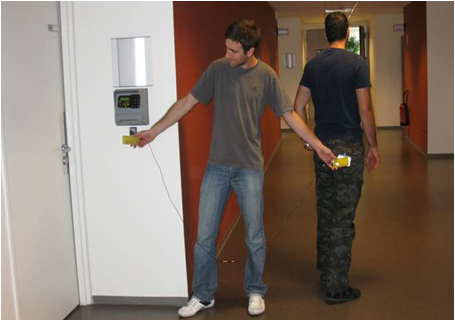
\includegraphics{relay-attack}
    \caption{\textbf{Relay attack} - Attack where an attacker authenticates by relaying the signal to the victim and replaying his response\cite{thevenon13}.}
\end{figure}
\begin{figure}[h!]
    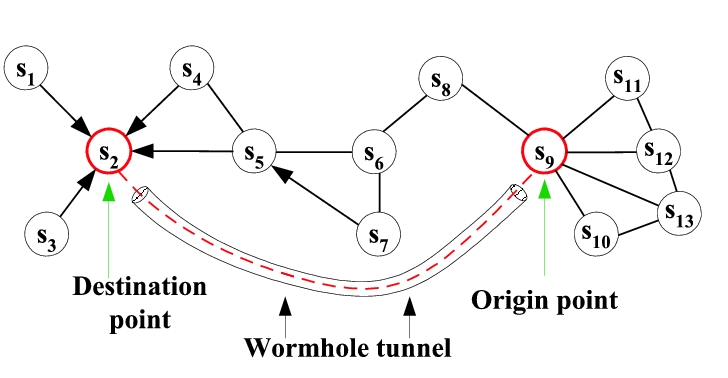
\includegraphics[width=1.0\textwidth]{wormhole-attack}
    \caption{\textbf{Wormhole attack} - A "wormhole" controlled by an attacker is set up between two networks. Due to a new shorter route being advertised, the wormhole will attract a considerable amount of traffic, which the attacker can drop, redirect or spy on depending on what he want to achieve\cite{infotec}.}
\end{figure}
\clearpage
\section{Solution}
\verb!T-protocols! A T-protocol is a protocol which tries to perform neighbour discovery using a timer which measures RTT. Unfortunately no such protocol can solve the secure neighbour discovery problem, since an adversary is indistinguishable from a correct node\cite{poturalski2013}.
\\
\\
Instead the scheme described in \cite{ShokriPRPH:C:09} solves the problem. The scheme is divided into three parts. The first part consists of measuring the distance $d_{ij}$ between each pair of nodes $(i, j)$ using ultra-sound. The second step consists of every node sharing a neighbour table containing the triples ($i$, $j$, $d_{ij}$). All messages are encrypted with a shared secret for confidentiality, and authenticated with MAC to detect tampering. The third and last step is called link verification, where three consistency tests are performed. If a node fails a consistency test, it is ignored and discarded.
\\
\\
The consistency tests for a node $i$ are as follows:
\begin{enumerate}
    \item \textbf{Link symmetry test} The distance between $i$ and $j$ must be equal to the distance between $j$ and $i$.
    \item \textbf{Maximum range test} The distance to a node must be within the communication range.
    \item \textbf{Quadrilateral test} For every neighbour $j$, find two other neighbours $u$ and $v$ such that $(i, j, u, v)$ are all neighbours and the polygon whose corners are the nodes $(i, j, u, v)$ is convex. A convex polygon is a polygon where all interior angles are $\le 180$ degrees. 
\end{enumerate}
\verb!Note! The last consistency test requires the location for each of the nodes. We must therefore combine this protocol with a protocol for secure location communication. To be continued...
\clearpage
\bibliographystyle{acm}
\bibliography{ref}
\end{document}